\documentclass[11pt,xcolor={dvipsnames},hyperref={pdftex,pdfpagemode=UseNone,hidelinks,pdfdisplaydoctitle=true},usepdftitle=false]{beamer}
\usepackage{presentation}
\usepackage{stmaryrd}

\hypersetup{pdftitle={Augmenting Model-Based Instantiation with Fast Enumeration}}
\newcommand\sym[1]{\mathsf{#1}}
\newcommand\ty[1]{\mathit{#1}}
\newcommand{\nt}[1]{\langle \mathsf{#1} \rangle}

\newcommand{\func}[1]{\ensuremath{\mathtt{#1}}\xspace}
\newcommand{\pt}{\phantom{0}}
\newcommand{\ptt}{\phantom{0}\phantom{0}}
\newcommand{\pttt}{\phantom{0}\phantom{0}\phantom{0}}
\newcommand{\ptttt}{\phantom{0}\phantom{0}\phantom{0}\phantom{0}}
\newcommand{\system}{\textsc{Goblin}}
\newcommand{\green}[1]{\textcolor{green!60!black}{#1}}
\newcommand{\red}[1]{\textcolor{red!70!black}{#1}}
\newcommand{\blue}[1]{\textcolor{blue!70!black}{#1}}
\newcommand{\teal}[1]{{\color{teal}{#1}}}
\newcommand{\highlight}{\makebox[0pt][l]{\color{lightgray}\rule[-2pt]{\linewidth}{9pt}}}
\definecolor{darkred}{rgb}{0.6,0.0,0.0} 
\definecolor{darkgreen}{RGB}{0,100,0}  
\definecolor{darkblue}{RGB}{0,0,175} 
\definecolor{lightgray}{gray}{0.85}

\newrobustcmd\B{\DeclareFontSeriesDefault[rm]{bf}{b}\bfseries} 
\usepackage{siunitx}
\usepackage{mathpartir} 
\usepackage{mdframed}
% \usepackage{algorithmicx}
% \usepackage{algpseudocode}
% \usepackage{algorithm}
% \usepackage[noend]{algorithmic}
\usepackage{algorithm}
\usepackage[noend]{algorithmic}
\usepackage[normalem]{ulem}
\usepackage{xcolor}
\usepackage{tikz}
\usepackage{listings}
\usepackage{xspace}
\newcommand{\code}[1]{{\footnotesize\texttt{#1}}}
\setbeamercovered{invisible}  
% Define a custom dark green color
\definecolor{darkgreen}{rgb}{0.0, 0.5, 0.0}
\usetikzlibrary{trees,arrows.meta,matrix,positioning,calc,fit,shapes.geometric,fit}
\lstdefinelanguage{plain}{
  sensitive=true,
  % morekeywords=[1]{int_to_bv,length,mod,seq,len,set,singleton,union,member},
  % morekeywords=[2]{BitVec,Int,Bool,List,Set,String},
  % morekeywords=[3]{bvand,bvor,bvxor,bvnot,and,or,not,bvplus,bvugt,bvult,bvmul}
}

\lstdefinestyle{plain}{
  language=plain,
  basicstyle=\ttfamily\scriptsize,
  numbers=left,
  numberstyle=\tiny\color{gray},
  xleftmargin=2.2em,
  linewidth=.97\columnwidth,
  stepnumber=1,
  frame=single,
  % framesep=4pt,
  showstringspaces=false,
  breaklines=true,
  tabsize=2,
  columns=fullflexible,
  commentstyle=\color{gray}\itshape,
  stringstyle=\color{red!70!black}, 
  % keywordstyle=[1]\color{blue},
  % keywordstyle=[2]\color{teal}\bfseries, 
  % keywordstyle=[3]\color{purple}\bfseries,
  keepspaces,
  escapeinside={@}{@},
  % moredelim=[is][\color{anglemark}\bfseries]{<}{>},
literate=% 
%     {0}{{{\color{darkred}0}}}1
%     {0b}{{{\color{darkred}0b}}}1
%     {1}{{{\color{darkred}1}}}1
%     {2}{{{\color{darkred}2}}}1
%     {3}{{{\color{darkred}3}}}1
%     {4}{{{\color{darkred}4}}}1
%     {5}{{{\color{darkred}5}}}1
%     {6}{{{\color{darkred}6}}}1
%     {7}{{{\color{darkred}7}}}1
%     {8}{{{\color{darkred}8}}}1
%     {9}{{{\color{darkred}9}}}1
%     % {.}{{{\color{blue}.}}}1
    {-->}{{{$\leadsto$}}}1
%     % {::}{{{\color{black}\bfseries ::}}}3%
%     % {=}{{{\color{black}\bfseries =}}}3%
%     % {<-}{{{\color{black}\bfseries <-}}}3%
%     % {+}{{{\color{black}\bfseries +}}}3%
%     % {|}{{{\color{black}\bfseries |}}}3%
%     % {;}{{{\color{black}\bfseries ;}}}3%
%     % {\{}{{{\color{black}\bfseries \{}}}3%
%     % {\}}{{{\color{black}\bfseries \}}}}3%
%     % {<}{{{\color{green}\bfseries <}}}3%
}
\algsetup{linenosize=\tiny}
\begin{document}
\lstdefinelanguage{Goblin}{
  sensitive=true,
  morekeywords=[1]{int_to_bv,length,mod,seq,len,set,singleton,union,member},
  morekeywords=[2]{BitVec,Int,Bool,List,Set,String},
  morekeywords=[3]{bvand,bvor,bvxor,bvnot,and,or,not,bvplus,bvugt,bvult,bvmul}
}

\lstdefinestyle{goblin}{
  language=Goblin,
  basicstyle=\ttfamily\scriptsize,
  numbers=left,
  numberstyle=\tiny\color{gray},
  xleftmargin=0em,
  stepnumber=1,
  frame=single,
  linewidth=.94\columnwidth,
  % framesep=4pt,
  showstringspaces=false,
  breaklines=true,
  tabsize=2,
  columns=fullflexible,
  commentstyle=\color{gray}\itshape,
  stringstyle=\color{red!70!black}, 
  keywordstyle=[1]\color{blue},
  keywordstyle=[2]\color{teal}\bfseries, 
  keywordstyle=[3]\color{purple}\bfseries,
  keepspaces,
  escapeinside={@}{@},
  % moredelim=[is][\color{anglemark}\bfseries]{<}{>},
literate=% 
    {0}{{{\color{darkred}0}}}1
    {0b}{{{\color{darkred}0b}}}1
    {1}{{{\color{darkred}1}}}1
    {2}{{{\color{darkred}2}}}1
    {3}{{{\color{darkred}3}}}1
    {4}{{{\color{darkred}4}}}1
    {5}{{{\color{darkred}5}}}1
    {6}{{{\color{darkred}6}}}1
    {7}{{{\color{darkred}7}}}1
    {8}{{{\color{darkred}8}}}1
    {9}{{{\color{darkred}9}}}1
    % {.}{{{\color{blue}.}}}1
    {-->}{{{$\leadsto$}}}1
    % {::}{{{\color{black}\bfseries ::}}}3%
    % {=}{{{\color{black}\bfseries =}}}3%
    % {<-}{{{\color{black}\bfseries <-}}}3%
    % {+}{{{\color{black}\bfseries +}}}3%
    % {|}{{{\color{black}\bfseries |}}}3%
    % {;}{{{\color{black}\bfseries ;}}}3%
    % {\{}{{{\color{black}\bfseries \{}}}3%
    % {\}}{{{\color{black}\bfseries \}}}}3%
    % {<}{{{\color{green}\bfseries <}}}3%
}


% \setstretch{1.25}
\setbeamerfont{title}{size=\Large}
\title{Parse this! \\ Summoning Context-Sensitive Inputs with \system{}}
%\subtitle{Extending SMT solving}

\information
%  
% []  
%
{\underline{Rob Lorch} \quad Muhammad Daniyal Pirwani Dar \newline \quad Cesare Tinelli \quad Omar Chowdhury
\newline \newline   
The University of Iowa
\newline    
Stony Brook University
}
%
%{TACAS 2025 \\2025-05-05, Hamilton, Canada}

\frame{\titlepage}

\begin{frame} 
    \frametitle{Problem Introduction} %\pause
    \begin{itemize}
        \item Some software systems have highly \green{complex input formats} (e.g. compilers, file renderers, network protocol stacks) \pause
        \item Complex input formats are difficult for testing, especially \green{automated testing} \pause
        \item We will discuss techniques for \green{automated input generation} of software with complex input formats \pause
        \item Given an input specification, how to generate inputs?
    \end{itemize}
    % What problem are we addressing?
    % Like paper introduction
    % Software sometimes has highly complex input formats, which are difficult for automated testing, 
    %   especially if blackbox
    % In general, we are interest in the problem of automated testing of software with highly complex
    %   input spec
    % More concretely, we focus on the problem of **input generation**
    %   - we have a spec and we want to generate inputs
\end{frame}

\begin{frame} 
    \frametitle{Existing Approaches} 
    \begin{itemize}
        \item Use \green{context-free grammars} (CFGs) to capture input structure \pause
        \begin{itemize}
            \item HTTP requests, DNS packets, LangFuzz\pause
            \item Can only handle context-free aspects of the spec\pause
            \item Consider packet format with fields 
            \blue{$f_1$} and \blue{$f_2$} s.t. \blue{$f_1 = |f_2|$}\pause
        \end{itemize}
        \item Tools tailor-made for \green{system under test} (SUT)\pause
        \begin{itemize}
            \item CSmith\pause
            \item Lacks generality!\pause
        \end{itemize}
        \item \green{Coverage-guided mutation}\pause
        \begin{itemize}
            \item How to generate an initial corpus?\pause
            \item What if no access to coverage information?\pause
            \item Mutations still blind to specification constraints
        \end{itemize}
    \end{itemize}
    % Conceptually different approaches
    % Context-free grammar based fuzzing (examples)
    % General-purpose code (a la CSmith, examples)
    % Coverage-guided mutation
        % - how to generate an initial corpus? Back to square 1
        % - what if you don't have access to coverage information?
        % - even so, mutations are blind to the input constraints, performance can be poor
    % Give negatives of all
\end{frame}

\begin{frame} 
    \frametitle{Wishlist} 
    \begin{enumerate}
        \item Generality of CFG-based approaches\pause
        \item Expressiveness of tailor-made fuzzers\pause
    \end{enumerate}
    \center{
    \textbf{Refine CFG-based approaches to be more expressive,} \newline 
    \textbf{while maintaining their generality}}
    % We want the generality of CFG-based approaches
    % We want the expressiveness of tailormade solutions
    % First basic idea: Refine CFG-based approaches to be more expressive, while maintaining their generality
\end{frame}

\begin{frame}[fragile]
    \frametitle{Context-free input generation} 
  First, a CFG-based input generation example: XML! \\[4pt]\pause
\begin{lstlisting}[style=goblin]
<xml-tree> ::= <openclose-tag> | 
               <open-tag> <inner-tree> <close-tag>
               
<inner-tree> ::= <TEXT> | <xml-tree> 
               | <inner-tree> <inner-tree> 
                     
<open-tag>  ::= `<'  <id> `>' | `<' <id> ` ' <attribute> `>'
<close-tag> ::= `</' <id> `>'

<openclose-tag> := `<' <id> `/>' 
                 | `<' <id> ` ' <attribute> `/>'

<attribute> ::= <id> `="' <TEXT > `"' 
              | <attribute> ` ' <attribute> 
                    
<id> ::= <ID-START-CHAR> <ID-CHAR>* 
\end{lstlisting}
\end{frame}

\begin{frame}[fragile]
    \frametitle{Context-free input generation} 
Termination? (Mostly) well-formed inputs?
\begin{lstlisting}[style=goblin]
<xml-tree> ::= <openclose-tag> | 
               <open-tag> <inner-tree> <close-tag>
               
<inner-tree> ::= <TEXT> | <xml-tree> 
               | <inner-tree> <inner-tree> 
                     
<open-tag>  ::= `<'  <id> `>' | `<' <id> ` ' <attribute> `>'
<close-tag> ::= `</' <id> `>'

<openclose-tag> := `<' <id> `/>' 
                 | `<' <id> ` ' <attribute> `/>'

<attribute> ::= <id> `="' <TEXT > `"' 
              | <attribute> ` ' <attribute> 
                    
<id> ::= <ID-START-CHAR> <ID-CHAR>* 
\end{lstlisting}
\end{frame}

\begin{frame}[fragile]
    \frametitle{Introducing \system{}} 
    \begin{itemize}
        \item Presenting \system{} \pause
        \begin{itemize}
        \item A \green{context-sensitive input generation tool}, supported by \pause
        \item A new \green{DSL} with a formal semantics \pause
        \item A new \green{search algorithm} to address the underlying problem \pause
        \item Supporting constraint solving over arbitrary SMT theories \pause
        \item And evaluated in the context of real fuzzing workflows \pause
        \end{itemize}
        \item Given a \green{context-sensitive grammar} \blue{$G$}, find \blue{$x$} such that \blue{$x \in \mathcal{L}(G)$} \pause
        \item What is a context-sensitive grammar? 
\begin{lstlisting}[style=goblin]
<xml-tree> ::= <openclose-tag> | 
               <open-tag> <inner-tree> <close-tag>
             @\blue{\{ <open-tag>.<id> = <close-tag>.<id> \}}@
... 
\end{lstlisting}
    \end{itemize}
    % Context-sensitive input generator
    % Specific example (eg XML) 
    %   - input is grammar + constraints, output is XML input
    % Generalization (CFG, constraints, Goblin, serializer, parser)
\end{frame}



\begin{frame}
    \frametitle{Input generation vs fuzzing} 
    \system{} is an \green{input generator}, but not a (complete) \green{fuzzer} \\[8pt]\pause
        \resizebox{\linewidth}{!}{
        {\scriptsize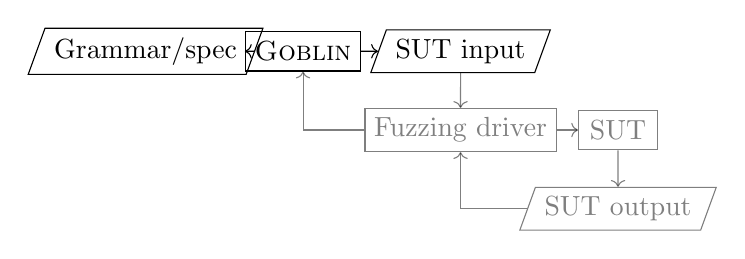
\begin{tikzpicture}[
            box/.style={draw, rectangle, minimum width=1cm, minimum height=.5cm, align=center},
            data/.style={draw, trapezium, trapezium left angle=70, trapezium right angle=110,
                 minimum width=1.2cm, minimum height=.5cm, align=center}
            ]
 
            % Nodes with manual coordinates
            \node[data] (inp) at (0,2) {Grammar/spec};
            \node[box] (sys) at (2,2) {\system{}};
            \node[data] (sutinp) at (4,2) {SUT input};
            \node[box][opacity=.5] (dr) at (4,1) {Fuzzing driver};
            \node[box][opacity=.5] (sut) at (6,1) {SUT};
            \node[data][opacity=.5] (sutout) at (6,0) {SUT output};

            % Arrows
            \draw[->] (inp.east) -- (sys.west);
            \draw[->] (sys.east) -- (sutinp.west);
            \draw[->][opacity=.5] (sutinp.south) -- (dr.north);
            \draw[->][opacity=.5] (dr.east) -- (sut.west);
            \draw[->][opacity=.5] (dr.west) -| (sys.south);
            \draw[->][opacity=.5] (sut.south) -- (sutout.north);
            \draw[->][opacity=.5] (sutout.west) -| (dr.south);
        \end{tikzpicture}}}
\end{frame}

\begin{frame}
    \frametitle{Input generation vs fuzzing} 
    \system{} is an \green{input generator}, but not a (complete) \green{fuzzer} \\[8pt]
        \resizebox{\linewidth}{!}{
        {\scriptsize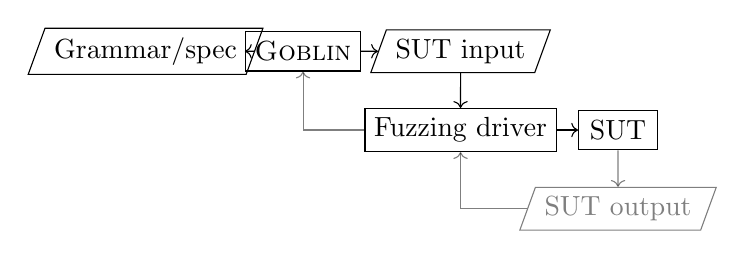
\begin{tikzpicture}[
            box/.style={draw, rectangle, minimum width=1cm, minimum height=.5cm, align=center},
            data/.style={draw, trapezium, trapezium left angle=70, trapezium right angle=110,
                 minimum width=1.2cm, minimum height=.5cm, align=center}
            ]
 
            % Nodes with manual coordinates
            \node[data] (inp) at (0,2) {Grammar/spec};
            \node[box] (sys) at (2,2) {\system{}};
            \node[data] (sutinp) at (4,2) {SUT input};
            \node[box] (dr) at (4,1) {Fuzzing driver};
            \node[box] (sut) at (6,1) {SUT};
            \node[data][opacity=.5] (sutout) at (6,0) {SUT output};

            % Arrows
            \draw[->] (inp.east) -- (sys.west);
            \draw[->] (sys.east) -- (sutinp.west);
            \draw[->] (sutinp.south) -- (dr.north);
            \draw[->] (dr.east) -- (sut.west);
            \draw[->][opacity=.5] (dr.west) -| (sys.south);
            \draw[->][opacity=.5] (sut.south) -- (sutout.north);
            \draw[->][opacity=.5] (sutout.west) -| (dr.south);
        \end{tikzpicture}}}
\end{frame}

\begin{frame}
    \frametitle{Input generation vs fuzzing} 
    \system{} is an \green{input generator}, but not a (complete) \green{fuzzer} \\[8pt]
        \resizebox{\linewidth}{!}{
        {\scriptsize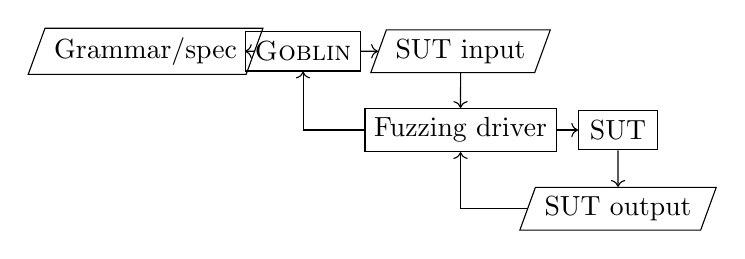
\begin{tikzpicture}[
            box/.style={draw, rectangle, minimum width=1cm, minimum height=.5cm, align=center},
            data/.style={draw, trapezium, trapezium left angle=70, trapezium right angle=110,
                 minimum width=1.2cm, minimum height=.5cm, align=center}
            ]
 
            % Nodes with manual coordinates
            \node[data] (inp) at (0,2) {Grammar/spec};
            \node[box] (sys) at (2,2) {\system{}};
            \node[data] (sutinp) at (4,2) {SUT input};
            \node[box] (dr) at (4,1) {Fuzzing driver};
            \node[box] (sut) at (6,1) {SUT};
            \node[data] (sutout) at (6,0) {SUT output};

            % Arrows
            \draw[->] (inp.east) -- (sys.west);
            \draw[->] (sys.east) -- (sutinp.west);
            \draw[->] (sutinp.south) -- (dr.north);
            \draw[->] (dr.east) -- (sut.west);
            \draw[->] (dr.west) -| (sys.south);
            \draw[->] (sut.south) -- (sutout.north);
            \draw[->] (sutout.west) -| (dr.south);
        \end{tikzpicture}}}
\end{frame}

\begin{frame}[fragile]
    \frametitle{\system{} by example: Language features}
\system{} grammars have \green{production rules} as in CFGs\\[4pt]
\begin{lstlisting}[style=goblin]
@\highlight@@\color{darkred}<PACKET>@ ::= @\color{teal}<TYPE>@ @\color{teal}<AUX>@ @\color{darkred}<PAYLOAD>@;



@\highlight@@\color{darkred}<PAYLOAD>@ ::= @\color{teal}<F1>@ @\color{teal}<F2>@ @\color{darkred}<BYTES>@; 

@\highlight@@\color{darkred}<BYTES>@ ::= @\color{teal}<BYTE>@ @\color{darkred}<BYTES>@ | @\color{teal}<BYTE>@ | @\color{teal}<OPT>@;



 @\;@
\end{lstlisting}
\end{frame}

\begin{frame}[fragile]
    \frametitle{\system{} by example: Language features}
Use \green{symbolic terminals} (in \teal {teal}) with \green{type annotations} rather than 
concrete terminals. Capture \green{abstract syntax}, not \green{concrete syntax}\\[4pt]
\begin{lstlisting}[style=goblin]
@\color{darkred}<PACKET>@ ::= @\color{teal}<TYPE>@ @\color{teal}<AUX>@ @\color{darkred}<PAYLOAD>@;



@\color{darkred}<PAYLOAD>@ ::= @\color{teal}<F1>@ @\color{teal}<F2>@ @\color{darkred}<BYTES>@; 

@\color{darkred}<BYTES>@ ::= @\color{teal}<BYTE>@ @\color{darkred}<BYTES>@ | @\color{teal}<BYTE>@ | @\color{teal}<OPT>@;
@\highlight@@\color{teal}<TYPE>@ :: BitVec(8);
@\highlight@@\color{teal}<BYTE>@ :: BitVec(8); 
@\highlight@@\color{teal}<AUX>@ :: BitVec(8); 
@\highlight@@\color{teal}<F1>@ :: BitVec(8); @\color{teal}<F2>@ :: BitVec(8); @\color{teal}<OPT>@ :: BitVec(4); 
\end{lstlisting}
\end{frame}

\begin{frame}[fragile]
    \frametitle{\system{} by example: Language features}
Constrain symbolic terminals with \green{refinement types}\\[4pt]
\begin{lstlisting}[style=goblin]
@\color{darkred}<PACKET>@ ::= @\color{teal}<TYPE>@ @\color{teal}<AUX>@ @\color{darkred}<PAYLOAD>@;



@\color{darkred}<PAYLOAD>@ ::= @\color{teal}<F1>@ @\color{teal}<F2>@ @\color{darkred}<BYTES>@; 

@\color{darkred}<BYTES>@ ::= @\color{teal}<BYTE>@ @\color{darkred}<BYTES>@ | @\color{teal}<BYTE>@ | @\color{teal}<OPT>@;
@\highlight@@\color{teal}<TYPE>@ :: BitVec(8) { @\color{teal}<TYPE>@ = 0x01 or @\color{teal}<TYPE>@ = 0x02; };   
@\highlight@@\color{teal}<BYTE>@ :: BitVec(8) { @\color{teal}<BYTE>@ bvult 0x88;}; 
@\color{teal}<AUX>@ :: BitVec(8); 
@\color{teal}<F1>@ :: BitVec(8); @\color{teal}<F2>@ :: BitVec(8); @\color{teal}<OPT>@ :: BitVec(4); 
\end{lstlisting}
\end{frame}

\begin{frame}[fragile]
    \frametitle{\system{} by example: Language features}
Attach \green{semantic constraits} to production rules

Support types/functions/predicates with \green{SMT-LIB} analogues\\[4pt]
\begin{lstlisting}[style=goblin]
@\color{darkred}<PACKET>@ ::= @\color{teal}<TYPE>@ @\color{teal}<AUX>@ @\color{darkred}<PAYLOAD>@
@\highlight@  { @\color{teal}<AUX>@ <- @\color{darkred}<PAYLOAD>@.@\color{teal}<F1>@ bvmul @\color{darkred}<PAYLOAD>@.@\color{teal}<F2>@;
@\highlight@    @\color{teal}<TYPE>@ = 0x01 => (@\color{darkred}<PAYLOAD>@.@\color{darkred}<BYTES>@.@\color{teal}<BYTE>@ bvugt 0x20 
@\highlight@                and @\color{darkred}<PAYLOAD>@.@\color{darkred}<BYTES>@.@\color{teal}<BYTE>@ bvult 0x7E); };
@\color{darkred}<PAYLOAD>@ ::= @\color{teal}<F1>@ @\color{teal}<F2>@ @\color{darkred}<BYTES>@ 
@\highlight@ { @\color{darkred}<BYTES>@.@\color{teal}<OPT>@ bvugt 0x0; };
@\color{darkred}<BYTES>@ ::= @\color{teal}<BYTE>@ @\color{darkred}<BYTES>@ | @\color{teal}<BYTE>@ | @\color{teal}<OPT>@;
@\color{teal}<TYPE>@ :: BitVec(8) { @\color{teal}<TYPE>@ = 0x01 or @\color{teal}<TYPE>@ = 0x02; };   
@\color{teal}<BYTE>@ :: BitVec(8) { @\color{teal}<BYTE>@ bvult 0x88;}; 
@\color{teal}<AUX>@ :: BitVec(8); 
@\color{teal}<F1>@ :: BitVec(8); @\color{teal}<F2>@ :: BitVec(8); @\color{teal}<OPT>@ :: BitVec(4); 
\end{lstlisting}
\end{frame}

\begin{frame}[fragile]
    \frametitle{\system{} by example: Language features}
Reference child nonterminals with \green{dot notation}\\[4pt]
\begin{lstlisting}[style=goblin]
@\color{darkred}<PACKET>@ ::= @\color{teal}<TYPE>@ @\color{teal}<AUX>@ @\color{darkred}<PAYLOAD>@
@\highlight@  { @\color{teal}<AUX>@ <- @\color{darkred}<PAYLOAD>@.@\color{teal}<F1>@ bvmul @\color{darkred}<PAYLOAD>@.@\color{teal}<F2>@;
@\highlight@    @\color{teal}<TYPE>@ = 0x01 => (@\color{darkred}<PAYLOAD>@.@\color{darkred}<BYTES>@.@\color{teal}<BYTE>@ bvugt 0x20 
@\highlight@                and @\color{darkred}<PAYLOAD>@.@\color{darkred}<BYTES>@.@\color{teal}<BYTE>@ bvult 0x7E); };
@\color{darkred}<PAYLOAD>@ ::= @\color{teal}<F1>@ @\color{teal}<F2>@ @\color{darkred}<BYTES>@ 
@\highlight@ { @\color{darkred}<BYTES>@.@\color{teal}<OPT>@ bvugt 0x0; };
@\color{darkred}<BYTES>@ ::= @\color{teal}<BYTE>@ @\color{darkred}<BYTES>@ | @\color{teal}<BYTE>@ | @\color{teal}<OPT>@;
@\color{teal}<TYPE>@ :: BitVec(8) { @\color{teal}<TYPE>@ = 0x01 or @\color{teal}<TYPE>@ = 0x02; };   
@\color{teal}<BYTE>@ :: BitVec(8) { @\color{teal}<BYTE>@ bvult 0x88;}; 
@\color{teal}<AUX>@ :: BitVec(8); 
@\color{teal}<F1>@ :: BitVec(8); @\color{teal}<F2>@ :: BitVec(8); @\color{teal}<OPT>@ :: BitVec(4); 
\end{lstlisting}
\end{frame}

\begin{frame}[fragile]
    \frametitle{\system{} by example: Language features}
Dot notation is \green{partial} and \green{implicitly universally quantified}\\[4pt]
\begin{lstlisting}[style=goblin]
@\color{darkred}<PACKET>@ ::= @\color{teal}<TYPE>@ @\color{teal}<AUX>@ @\color{darkred}<PAYLOAD>@
  { @\color{teal}<AUX>@ <- @\color{darkred}<PAYLOAD>@.@\color{teal}<F1>@ bvmul @\color{darkred}<PAYLOAD>@.@\color{teal}<F2>@;
    @\color{teal}<TYPE>@ = 0x01 => (@\color{darkred}<PAYLOAD>@.@\color{darkred}<BYTES>@.@\color{teal}<BYTE>@ bvugt 0x20 
                and @\color{darkred}<PAYLOAD>@.@\color{darkred}<BYTES>@.@\color{teal}<BYTE>@ bvult 0x7E); };
@\color{darkred}<PAYLOAD>@ ::= @\color{teal}<F1>@ @\color{teal}<F2>@ @\color{darkred}<BYTES>@ 
@\highlight@ { @\color{darkred}<BYTES>@.@\color{teal}<OPT>@ bvugt 0x0; };
@\color{darkred}<BYTES>@ ::= @\color{teal}<BYTE>@ @\color{darkred}<BYTES>@ | @\color{teal}<BYTE>@ | @\color{teal}<OPT>@;
@\color{teal}<TYPE>@ :: BitVec(8) { @\color{teal}<TYPE>@ = 0x01 or @\color{teal}<TYPE>@ = 0x02; };   
@\color{teal}<BYTE>@ :: BitVec(8) { @\color{teal}<BYTE>@ bvult 0x88;}; 
@\color{teal}<AUX>@ :: BitVec(8); 
@\color{teal}<F1>@ :: BitVec(8); @\color{teal}<F2>@ :: BitVec(8); @\color{teal}<OPT>@ :: BitVec(4); 
\end{lstlisting}
\end{frame}

\begin{frame}[fragile]
    \frametitle{\system{} by example: Language features}
Many constraints are not amenable to \green{automated constraint solving} 
with an \green{SMT engine}\\[4pt]
\begin{lstlisting}[style=goblin]
@\color{darkred}<PACKET>@ ::= @\color{teal}<TYPE>@ @\color{teal}<AUX>@ @\color{darkred}<PAYLOAD>@
@\highlight@  { @\color{teal}<AUX>@ <- @\color{darkred}<PAYLOAD>@.@\color{teal}<F1>@ bvmul @\color{darkred}<PAYLOAD>@.@\color{teal}<F2>@;
...
@\color{darkred}<PAYLOAD>@ ::= @\color{teal}<F1>@ @\color{teal}<F2>@ @\color{darkred}<BYTES>@ 
...
\end{lstlisting}\pause
\green{Derived fields} with \blue{\scriptsize\texttt{<-}} denote nonterminals that are directly computable, enforced syntactically \pause

Cryptographic hashes, checksums, or \green{any computable function}
\end{frame}

\tikzset{
  >=Latex,                             % nice arrowheads
  proc/.style = {draw, rounded corners, thick, fill=white, inner sep=6pt, minimum width=2cm, align=center},
  flow/.style = {->, thick},           % arrow style
  lab/.style  = {font=\small, midway, above} % label style
  io/.style   = {proc, trapezium, trapezium stretches=true,
                 trapezium left angle=70, trapezium right angle=110,
                 fill=gray!15, very thick}
} 
\begin{frame} 
    \frametitle{Semantics: Abstract syntax trees}
% \begin{itemize}
    \system{} generates \green{abstract syntax trees}, not strings\pause
%     \item AST view with SMT-LIB types enables constraint solving over SMT theories 
%     (prior work only natively supports string constraints)
% \end{itemize}


\newcommand{\dttree}{%
    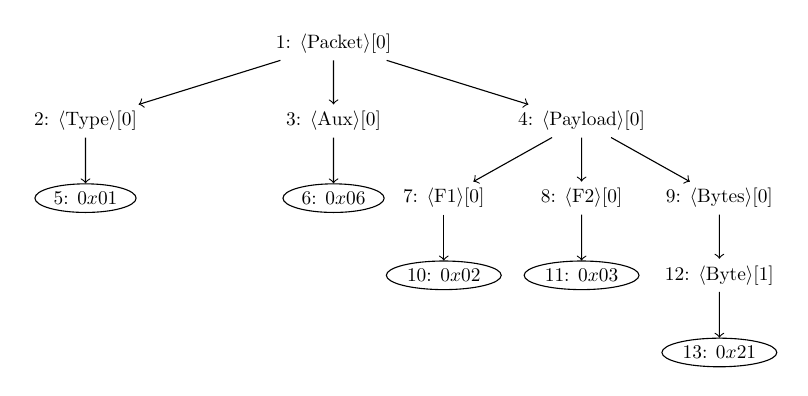
\begin{tikzpicture}[
      scale=0.7, transform shape,
      level distance=14mm,
      level 1/.style={sibling distance=45mm},
      level 2/.style={sibling distance=25mm},
      leaf/.style={draw, ellipse, inner sep=2pt}
    ]
      \node {1: $\langle$Packet$\rangle[0]$} [-to]
        child { node {2: $\langle$Type$\rangle[0]$}
          child { node[leaf] {5: $0x01$} }}
        child { node {3: $\langle$Aux$\rangle[0]$}
          child { node[leaf] {6: $0x06$} } }
        child { node {4: $\langle$Payload$\rangle[0]$} 
          child { node {7: $\langle$F1$\rangle[0]$} child { node[leaf] {10: $0x02$} } }
          child { node {8: $\langle$F2$\rangle[0]$} child { node[leaf] {11: $0x03$} } }
          child { node {9: $\langle$Bytes$\rangle[0]$} child { node {12: $\langle$Byte$\rangle[1]$} child { node[leaf] {13: $0x21$} } } } };
    \end{tikzpicture}%
  }
  {\center \dttree} \pause 

  \green{Not} a string \blue{{\scriptsize \texttt{0x0106020321}}}
% Grammar producing a string vs grammar producing an ADT term
% In the ADT view, we model derivations in progress as derivation trees
% Informally, the semantics of a Goblin input is the set of closed derivation trees 
%   that (i)  respect the context-free grammar rules and 
%        (ii) satisfy the constraints at every production rule application
\end{frame}

\begin{frame}
    \frametitle{Semantics: Abstract syntax trees}
    \begin{itemize}
        \item Without the AST view, prior work natively \green{only supports string constraints} \pause
        \item AST semantics position \system{} as a generator of constrained \green{algebraic datatype} (ADT) terms\pause
    \end{itemize}
    \center {\textbf{The ADT view allows \system{} to natively support constraints over arbitrary SMT theories}}
\end{frame}

\begin{frame} 
    \frametitle{Semantics}
    The \green{semantics} of a goblin input \blue{$G$} are the set of ASTs that 
    respect $(i)$ \blue{$G$}'s context-free syntactic constraints and \blue{$G$}'s 
    $(ii)$ context-sensitive semantic constraints \pause 

    \blue{$\mathcal{L}_{\mathsf{AST}}(G) = \{ t \mid $}
\begin{enumerate}
    \item \blue{$t$} is rooted at the start symbol\pause
    \item Each \blue{$v \in V(t)$} is either \pause
    \begin{enumerate}
        \item A non-leaf with children representing a production rule application in \blue{$G$},\pause
        \item A non-leaf representing a type annotation in \blue{$G$}, or\pause
        \item A well-typed leaf\pause
    \end{enumerate}
    \item \blue{$t$} satisfies the constraints at every production rule application
\end{enumerate}
    \blue{$\}$}
\end{frame}

\begin{frame} [fragile]
    \frametitle{Semantics: Constraint Satisfaction}
 \begin{lstlisting}[style=goblin]
@\color{darkred}<PACKET>@ ::= @\color{teal}<TYPE>@ @\color{teal}<AUX>@ @\color{darkred}<PAYLOAD>@
@\highlight@  { @\color{teal}<AUX>@ <- @\color{darkred}<PAYLOAD>@.@\color{teal}<F1>@ bvmul @\color{darkred}<PAYLOAD>@.@\color{teal}<F2>@;
...
@\color{darkred}<PAYLOAD>@ ::= @\color{teal}<F1>@ @\color{teal}<F2>@ @\color{darkred}<BYTES>@ 
...
\end{lstlisting}

\newcommand{\dttree}{%
    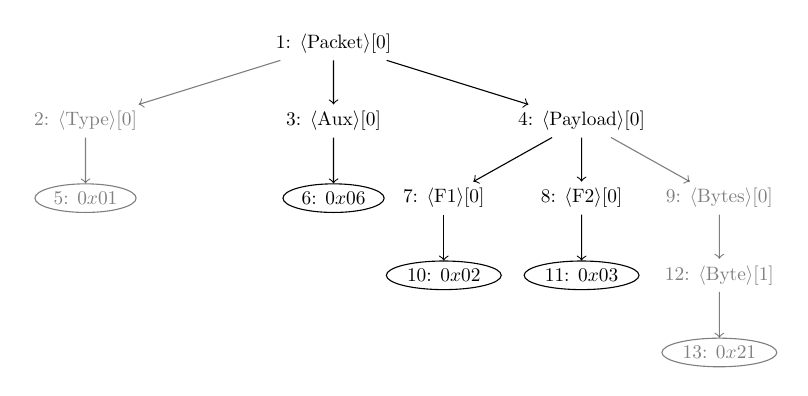
\begin{tikzpicture}[
      scale=0.7, transform shape,
      level distance=14mm,
      level 1/.style={sibling distance=45mm},
      level 2/.style={sibling distance=25mm},
      leaf/.style={draw, ellipse, inner sep=2pt}
    ]
      \node {1: $\langle$Packet$\rangle[0]$} [-to]
        child[opacity=.5] { node {2: $\langle$Type$\rangle[0]$}
          child { node[leaf] {5: $0x01$} }}
        child { node {3: $\langle$Aux$\rangle[0]$}
          child { node[leaf] {6: $0x06$} } }
        child { node {4: $\langle$Payload$\rangle[0]$} 
          child { node {7: $\langle$F1$\rangle[0]$} child { node[leaf] {10: $0x02$} } }
          child { node {8: $\langle$F2$\rangle[0]$} child { node[leaf] {11: $0x03$} } }
          child[opacity=.5] { node {9: $\langle$Bytes$\rangle[0]$} child { node {12: $\langle$Byte$\rangle[1]$} child { node[leaf] {13: $0x21$} } } } };
    \end{tikzpicture}%
  }
  {\center \dttree}
\end{frame}

\begin{frame} [fragile]
    \frametitle{Semantics: Constraint Satisfaction}
 \begin{lstlisting}[style=goblin]
...
@\color{teal}<BYTE>@ :: BitVec(8) { @\color{teal}<BYTE>@ bvult 0x88; }; 
...
\end{lstlisting}

\newcommand{\dttree}{%
    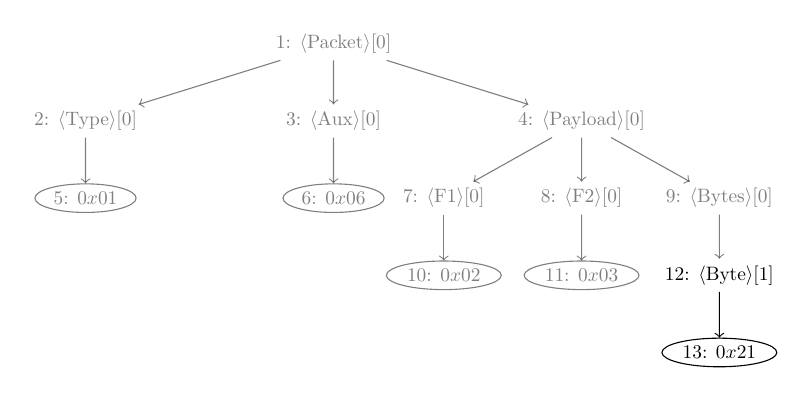
\begin{tikzpicture}[
      scale=0.7, transform shape,
      level distance=14mm,
      level 1/.style={sibling distance=45mm},
      level 2/.style={sibling distance=25mm},
      leaf/.style={draw, ellipse, inner sep=2pt}
    ]
      \node[opacity=.5] {1: $\langle$Packet$\rangle[0]$} [-to]
        child[opacity=.5] { node {2: $\langle$Type$\rangle[0]$}
          child { node[leaf] {5: $0x01$} }}
        child[opacity=.5] { node {3: $\langle$Aux$\rangle[0]$}
          child { node[leaf] {6: $0x06$} } }
        child[opacity=.5] { node {4: $\langle$Payload$\rangle[0]$} 
          child { node {7: $\langle$F1$\rangle[0]$} child { node[leaf] {10: $0x02$} } }
          child { node {8: $\langle$F2$\rangle[0]$} child { node[leaf] {11: $0x03$} } }
          child { node {9: $\langle$Bytes$\rangle[0]$} child { node[opacity=1] {12: $\langle$Byte$\rangle[1]$} child[opacity=1] { node[leaf] {13: $0x21$} } } } };
    \end{tikzpicture}%
  }
  {\center \dttree}
\end{frame}

\begin{frame} 
    \frametitle{\system{} Workflow}
    How does \system{} find \blue{$t$} such that \blue{$t \in \mathcal{L}_{\textsf{AST}}(G)$}?\\[4pt]\pause

    General workflow:\pause
    \begin{enumerate}
        \item \green{Context-free wellformedness} and other syntactic checks\pause
        \item Type checking\pause
        \item Desugar refinement types\pause
        \item Disambiguate constraints \pause
        \item \green{Abstract derived fields}\pause
        \item \green{Main search algorithm}\pause
        \item Compute derived fields\pause
        \item Serialize
    \end{enumerate}
    % Mention serialization step
\end{frame}

\begin{frame}[fragile]
    \frametitle{Context-Free Wellformedness}
    \begin{itemize}
        \item \green{Context-free language emptiness} (e.g., \blue{$S \rightarrow S$}) is a modeling issue, stemming from 
        \green{non-wellfounded recursion} \pause
        \item We perform a more general check called \green{context-free wellformedness}\pause
        \item[1.]  Iteratively expand a set \blue{$N$} of nonterminals known to be able to produce finite derivations 
        until reaching a fixpoint\pause
        \item[2.] Check every reachable nonterminal is in \blue{$N$}\pause
    \end{itemize}
\begin{lstlisting}[style=goblin]
@\color{darkred}<SAE\_PACKET>@ ::= @\color{darkred}<COMMIT>@ | @\color{darkred}<CONFIRM>@;
@\color{darkred}<COMMIT>@ ::= @\color{teal}<FIELD>@ @\color{darkred}<RG\_ID\_LIST>@;
@\highlight@@\color{darkred}<RG\_ID\_LIST>@ ::= @\color{teal}<RG\_ID>@ @\color{darkred}<RG\_ID\_LIST>@;
@\color{darkred}<CONFIRM>@ ::= @\color{teal}<FIELD1> <FIELD2>@;
...
\end{lstlisting}
\end{frame}

\begin{frame}
    \frametitle{Derived Field Checks}
    Derived fields \blue{$\langle F \rangle \leftarrow e$} must be computable \green{without constraint solving}\pause
    \begin{itemize}
        \item[1.] Disallow \green{cyclic dependencies} (e.g. \blue{$\langle A \rangle \rightarrow T[\langle B\rangle], \langle B\rangle \rightarrow T[\langle A\rangle]$})\pause
        \begin{itemize}
            \item[$(i)$] Build a directed graph for each prod rule\pause
            \item[$(ii)$] Include vertex for each RHS nonterminal/symbolic terminal\pause
            \item[$(iii)$] Check for cycles\pause
        \end{itemize}
        \item[2.] Disallow derived fields in semantic constraints\pause
        \begin{itemize}
            \item E.g., \blue{$\langle D \rangle > 0$} where \blue{$\langle D \rangle$} is derived
        \end{itemize}
    \end{itemize}
\end{frame}

\begin{frame}[fragile]
    \frametitle{Abstract derived fields}
We remove derived fields from $G$ before the main search; 
compute them after constraint solving\pause
\begin{lstlisting}[style=goblin]
@\color{darkred}<PACKET>@ ::= @\color{teal}<TYPE>@ @\color{teal}<AUX>@ @\color{darkred}<PAYLOAD>@
  { @\color{teal}<AUX>@ <- @\color{darkred}<PAYLOAD>@.@\color{teal}<F1>@ bvmul @\color{darkred}<PAYLOAD>@.@\color{teal}<F2>@;
...
\end{lstlisting}
\blue{$\leadsto$}
\begin{lstlisting}[style=goblin]
@\color{darkred}<PACKET>@ ::= @\color{teal}<TYPE>@ dep_sym_leaf @\color{darkred}<PAYLOAD>@
  { ...
\end{lstlisting}
\end{frame}

\begin{frame}[fragile]
    \frametitle{Search Algorithm: Main Concepts}
Start with \green{context-free case}

A \green{derivation tree} is an AST that may be \green{open} (or \green{closed})
\begin{enumerate}
\item Build candidate \blue{$\mathit{dt}$} via random walk until closed
\item Then instantiate with concrete values 
\end{enumerate}


 % --- helper: two derivation trees of different heights ---
\newcommand{\dttree}{%
  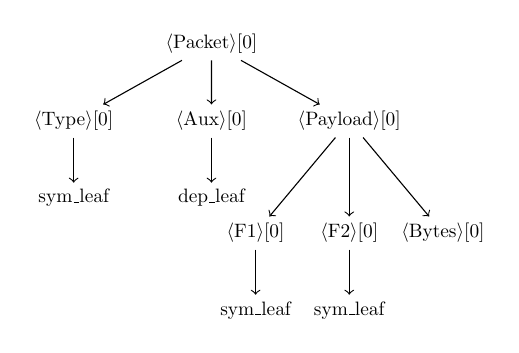
\begin{tikzpicture}[
    scale=0.7, transform shape,
    level distance=14mm,
    level 1/.style={sibling distance=25mm},
    level 2/.style={sibling distance=17mm},
    baseline=(current bounding box.center),
  ]
    \node {$\langle$Packet$\rangle[0]$} [-to]
      child { node {$\langle$Type$\rangle[0]$}
        child { node {sym\_leaf} }}
      child { node {$\langle$Aux$\rangle[0]$}
        child { node {dep\_leaf} } }
      child { node {$\langle$Payload$\rangle[0]$} 
        child { node[yshift=-18pt] {$\langle$F1$\rangle[0]$} 
          child { node {sym\_leaf} } }
        child { node[yshift=-18pt] {$\langle$F2$\rangle[0]$} 
          child { node {sym\_leaf} }}
        child { node[yshift=-18pt] {$\langle$Bytes$\rangle[0]$} }};
  \end{tikzpicture}%
}

\newcommand{\dttreee}{%
  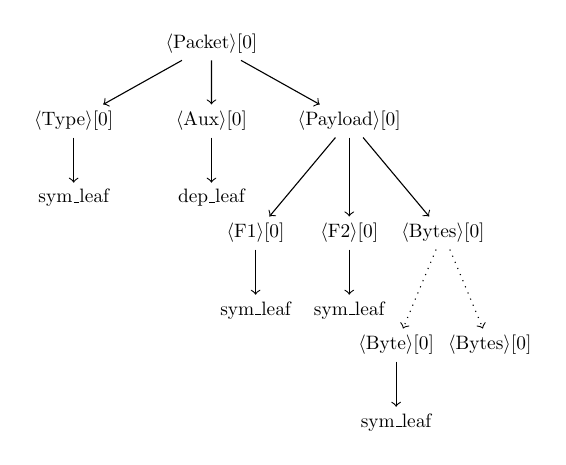
\begin{tikzpicture}[
    scale=0.7, transform shape,
    level distance=14mm,
    % root children (Type, Aux, Payload)
    level 1/.style={sibling distance=25mm},
    % children of Payload (F1, F2, Bytes)
    level 2/.style={sibling distance=17mm},
    % children of Bytes (Byte, Bytes)
    level 3/.style={sibling distance=17mm},
    baseline=(current bounding box.center),
  ]
    \node {$\langle$Packet$\rangle[0]$} [-to]
      child { node {$\langle$Type$\rangle[0]$}
        child { node {sym\_leaf} }}
      child { node {$\langle$Aux$\rangle[0]$}
        child { node {dep\_leaf} } }
      child { node {$\langle$Payload$\rangle[0]$} 
        child { node[yshift=-18pt] {$\langle$F1$\rangle[0]$} 
          child { node {sym\_leaf} } }
        child { node[yshift=-18pt] {$\langle$F2$\rangle[0]$} 
          child { node {sym\_leaf} }}
        child { node[yshift=-18pt] {$\langle$Bytes$\rangle[0]$} 
          % shift children of Bytes down to elongate arrows
          child[-to,dotted] { node[yshift=-18pt] {$\langle$Byte$\rangle[0]$}
            % this edge stays solid 
            child[-to,solid] { node {sym\_leaf} } }
          child[-to,dotted] { node[yshift=-18pt] {$\langle$Bytes$\rangle[0]$} } }
      };
  \end{tikzpicture}%
}

\begin{center}
\resizebox{\textwidth}{!}{%
\resizebox{\textwidth}{!}{%
  \begin{tabular}{c c c}
    \dttree & $\leadsto$ & \dttreee \\ 
    \blue{$dt_1$} & & \blue{$dt_2$}
  \end{tabular}
}
}
\end{center}
\end{frame}

\begin{frame}[fragile]
    \frametitle{Search Algorithm: Main Concepts}
Choosing an expansion is called a \green{decision}

Decisions are recorded in a \green{decision stack} \blue{$ds = [dt_1, dt_2]$}

 % --- helper: two derivation trees of different heights ---
\newcommand{\dttree}{%
  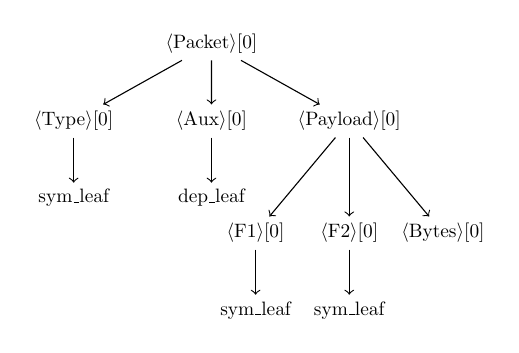
\begin{tikzpicture}[
    scale=0.7, transform shape,
    level distance=14mm,
    level 1/.style={sibling distance=25mm},
    level 2/.style={sibling distance=17mm},
    baseline=(current bounding box.center),
  ]
    \node {$\langle$Packet$\rangle[0]$} [-to]
      child { node {$\langle$Type$\rangle[0]$}
        child { node {sym\_leaf} }}
      child { node {$\langle$Aux$\rangle[0]$}
        child { node {dep\_leaf} } }
      child { node {$\langle$Payload$\rangle[0]$} 
        child { node[yshift=-18pt] {$\langle$F1$\rangle[0]$} 
          child { node {sym\_leaf} } }
        child { node[yshift=-18pt] {$\langle$F2$\rangle[0]$} 
          child { node {sym\_leaf} }}
        child { node[yshift=-18pt] {$\langle$Bytes$\rangle[0]$} }};
  \end{tikzpicture}%
}

\newcommand{\dttreee}{%
  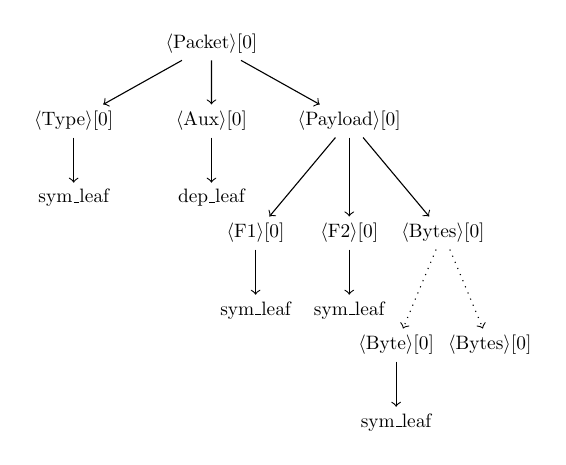
\begin{tikzpicture}[
    scale=0.7, transform shape,
    level distance=14mm,
    % root children (Type, Aux, Payload)
    level 1/.style={sibling distance=25mm},
    % children of Payload (F1, F2, Bytes)
    level 2/.style={sibling distance=17mm},
    % children of Bytes (Byte, Bytes)
    level 3/.style={sibling distance=17mm},
    baseline=(current bounding box.center),
  ]
    \node {$\langle$Packet$\rangle[0]$} [-to]
      child { node {$\langle$Type$\rangle[0]$}
        child { node {sym\_leaf} }}
      child { node {$\langle$Aux$\rangle[0]$}
        child { node {dep\_leaf} } }
      child { node {$\langle$Payload$\rangle[0]$} 
        child { node[yshift=-18pt] {$\langle$F1$\rangle[0]$} 
          child { node {sym\_leaf} } }
        child { node[yshift=-18pt] {$\langle$F2$\rangle[0]$} 
          child { node {sym\_leaf} }}
        child { node[yshift=-18pt] {$\langle$Bytes$\rangle[0]$} 
          % shift children of Bytes down to elongate arrows
          child[-to,dotted] { node[yshift=-18pt] {$\langle$Byte$\rangle[0]$}
            % this edge stays solid 
            child[-to,solid] { node {sym\_leaf} } }
          child[-to,dotted] { node[yshift=-18pt] {$\langle$Bytes$\rangle[0]$} } }
      };
  \end{tikzpicture}%
}

\begin{center}
\resizebox{\textwidth}{!}{%
\resizebox{\textwidth}{!}{%
  \begin{tabular}{c c c}
    \dttree & $\leadsto$ & \dttreee \\ 
    \blue{$dt_1$} & & \blue{$dt_2$}
  \end{tabular}
}
}
\end{center}
\end{frame}

\begin{frame}[fragile]
    \frametitle{Search Algorithm: Main Concepts}
Some ``decisions'' are \green{forced}: symbolic terminals and 
nonterminals with exactly one production rule option

These are called \green{normalization steps} and are not stored in \blue{$ds$}


 % --- helper: two derivation trees of different heights ---
\newcommand{\dttree}{%
  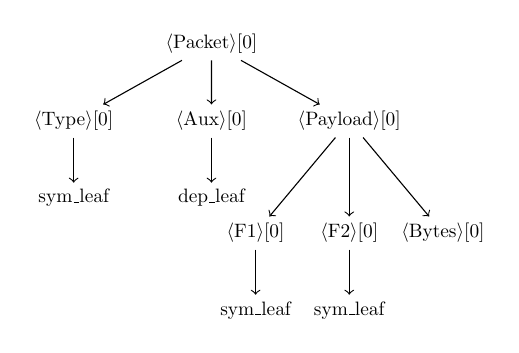
\begin{tikzpicture}[
    scale=0.7, transform shape,
    level distance=14mm,
    level 1/.style={sibling distance=25mm},
    level 2/.style={sibling distance=17mm},
    baseline=(current bounding box.center),
  ]
    \node {$\langle$Packet$\rangle[0]$} [-to]
      child { node {$\langle$Type$\rangle[0]$}
        child { node {sym\_leaf} }}
      child { node {$\langle$Aux$\rangle[0]$}
        child { node {dep\_leaf} } }
      child { node {$\langle$Payload$\rangle[0]$} 
        child { node[yshift=-18pt] {$\langle$F1$\rangle[0]$} 
          child { node {sym\_leaf} } }
        child { node[yshift=-18pt] {$\langle$F2$\rangle[0]$} 
          child { node {sym\_leaf} }}
        child { node[yshift=-18pt] {$\langle$Bytes$\rangle[0]$} }};
  \end{tikzpicture}%
}

\newcommand{\dttreee}{%
  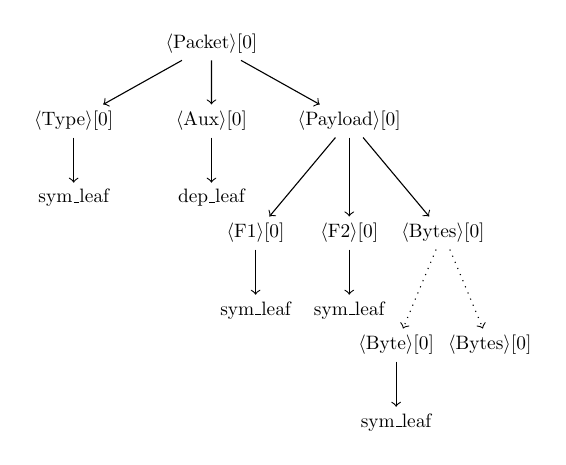
\begin{tikzpicture}[
    scale=0.7, transform shape,
    level distance=14mm,
    % root children (Type, Aux, Payload)
    level 1/.style={sibling distance=25mm},
    % children of Payload (F1, F2, Bytes)
    level 2/.style={sibling distance=17mm},
    % children of Bytes (Byte, Bytes)
    level 3/.style={sibling distance=17mm},
    baseline=(current bounding box.center),
  ]
    \node {$\langle$Packet$\rangle[0]$} [-to]
      child { node {$\langle$Type$\rangle[0]$}
        child { node {sym\_leaf} }}
      child { node {$\langle$Aux$\rangle[0]$}
        child { node {dep\_leaf} } }
      child { node {$\langle$Payload$\rangle[0]$} 
        child { node[yshift=-18pt] {$\langle$F1$\rangle[0]$} 
          child { node {sym\_leaf} } }
        child { node[yshift=-18pt] {$\langle$F2$\rangle[0]$} 
          child { node {sym\_leaf} }}
        child { node[yshift=-18pt] {$\langle$Bytes$\rangle[0]$} 
          % shift children of Bytes down to elongate arrows
          child[-to,dotted] { node[yshift=-18pt] {$\langle$Byte$\rangle[0]$}
            % this edge stays solid 
            child[-to,solid] { node {sym\_leaf} } }
          child[-to,dotted] { node[yshift=-18pt] {$\langle$Bytes$\rangle[0]$} } }
      };
  \end{tikzpicture}%
}

\begin{center}
\resizebox{\textwidth}{!}{%
\resizebox{\textwidth}{!}{%
  \begin{tabular}{c c c}
    \dttree & $\leadsto$ & \dttreee \\ 
    \blue{$dt_1$} & & \blue{$dt_2$}
  \end{tabular}
}
}
\end{center}
\end{frame}

\begin{frame}[fragile]
    \frametitle{Search Algorithm: Main Concepts}
\green{Termination} is not guaranteed

Pick a \green{depth limit} \blue{$L$} and associate a \green{search depth} with each \blue{$dt$}

\green{Backtrack} once \blue{$L$} is exceeded by popping \blue{$ds$}

Record visited expansions and do not revisit

\green{Restart} and increment \blue{$L$} if backtracking and \blue{$ds = []$}

 % --- helper: two derivation trees of different heights ---
\newcommand{\dttree}{%
  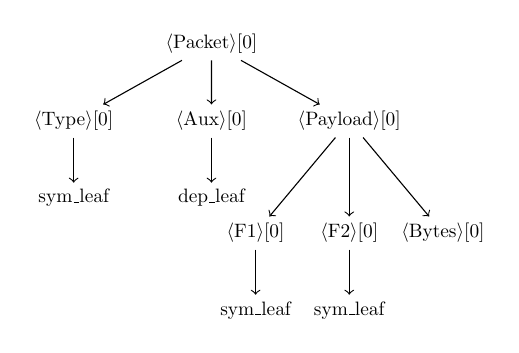
\begin{tikzpicture}[
    scale=0.7, transform shape,
    level distance=14mm,
    level 1/.style={sibling distance=25mm},
    level 2/.style={sibling distance=17mm},
    baseline=(current bounding box.center),
  ]
    \node {$\langle$Packet$\rangle[0]$} [-to]
      child { node {$\langle$Type$\rangle[0]$}
        child { node {sym\_leaf} }}
      child { node {$\langle$Aux$\rangle[0]$}
        child { node {dep\_leaf} } }
      child { node {$\langle$Payload$\rangle[0]$} 
        child { node[yshift=-18pt] {$\langle$F1$\rangle[0]$} 
          child { node {sym\_leaf} } }
        child { node[yshift=-18pt] {$\langle$F2$\rangle[0]$} 
          child { node {sym\_leaf} }}
        child { node[yshift=-18pt] {$\langle$Bytes$\rangle[0]$} }};
  \end{tikzpicture}%
}

\newcommand{\dttreee}{%
  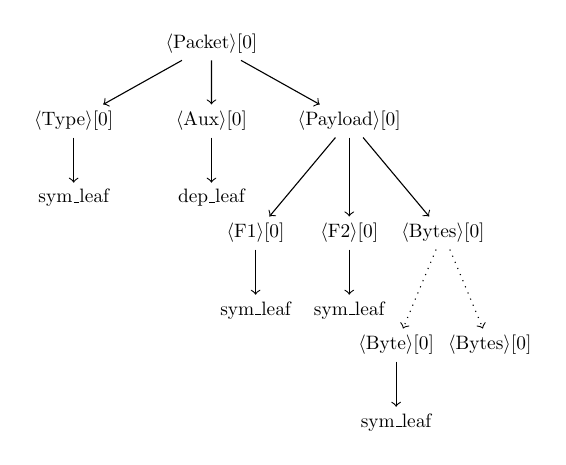
\begin{tikzpicture}[
    scale=0.7, transform shape,
    level distance=14mm,
    % root children (Type, Aux, Payload)
    level 1/.style={sibling distance=25mm},
    % children of Payload (F1, F2, Bytes)
    level 2/.style={sibling distance=17mm},
    % children of Bytes (Byte, Bytes)
    level 3/.style={sibling distance=17mm},
    baseline=(current bounding box.center),
  ]
    \node {$\langle$Packet$\rangle[0]$} [-to]
      child { node {$\langle$Type$\rangle[0]$}
        child { node {sym\_leaf} }}
      child { node {$\langle$Aux$\rangle[0]$}
        child { node {dep\_leaf} } }
      child { node {$\langle$Payload$\rangle[0]$} 
        child { node[yshift=-18pt] {$\langle$F1$\rangle[0]$} 
          child { node {sym\_leaf} } }
        child { node[yshift=-18pt] {$\langle$F2$\rangle[0]$} 
          child { node {sym\_leaf} }}
        child { node[yshift=-18pt] {$\langle$Bytes$\rangle[0]$} 
          % shift children of Bytes down to elongate arrows
          child[-to,dotted] { node[yshift=-18pt] {$\langle$Byte$\rangle[0]$}
            % this edge stays solid 
            child[-to,solid] { node {sym\_leaf} } }
          child[-to,dotted] { node[yshift=-18pt] {$\langle$Bytes$\rangle[0]$} } }
      };
  \end{tikzpicture}%
}

\begin{center}
\resizebox{\textwidth}{!}{%
\resizebox{\textwidth}{!}{%
  \begin{tabular}{c c c}
    \dttree & $\leadsto$ & \dttreee 
  \end{tabular}
}
}
\end{center}
\end{frame}

\begin{frame} \frametitle{Search Algorithm: Main Concepts}
    How to extend the context-free algorithm to handle constraints?\\[4pt]\pause
    
    Insight: use an \green{incremental SMT} backend\\[4pt]\pause

    Solver interface\pause
    \begin{itemize} 
      \item {\scriptsize\blue{\texttt{(assert c)}}}: assert a constraint\pause
      \item {\scriptsize\blue{\texttt{(push 1)}}}: push an assertion level\pause
      \item {\scriptsize\blue{\texttt{(pop 1)}}}: undo assertions in last assertion level (backtrack)\pause
      \item {\scriptsize\blue{\texttt{(check-sat)}}}: check if conjunction of active assertions is \blue{\textsc{SAT}}\pause
      \item {\scriptsize\blue{\texttt{(get-model)}}}: retrieve a concrete model
    \end{itemize}
\end{frame}

\begin{frame} \frametitle{Search Algorithm: Main Concepts}
    Principles of constraint handling\pause

    \begin{enumerate}
      \item Push an assertion frame at every decision\pause
      \item At each decision, {\scriptsize\blue{\texttt{assert}}} all constraints associated with the expanded \blue{$dt$} node and call {\scriptsize\blue{\texttt{check-sat}}}\pause
      \item Backtrack and pop an assertion level if {\scriptsize\blue{\texttt{check-sat}}} yields \blue{\textsc{Unsat}}\pause
      \item Do not commit to concrete values; call {\scriptsize\blue{\texttt{get-model}}} once \blue{$dt$} is closed
    \end{enumerate}
\end{frame}

\begin{frame}[fragile] \frametitle{Search Algorithm: Main concepts}
    There are wrinkles...\pause
\vspace{-4pt}
    \begin{enumerate}

    \item Constraints must be \green{disambiguated} and \green{universalized}\pause
    \end{enumerate}

\begin{lstlisting}[style=goblin]
@\color{darkred}<PACKET>@ ::= @\color{teal}<TYPE>@ @\color{teal}<AUX>@ @\color{darkred}<PAYLOAD>@ { ... };
@\color{darkred}<PAYLOAD>@ ::= @\color{teal}<F1>@ @\color{teal}<F2>@ @\color{darkred}<BYTES>@ 
@\highlight@ { @\color{darkred}<BYTES>@.@\color{teal}<OPT>@ bvugt 0x0; };
@\color{darkred}<BYTES>@ ::= @\color{teal}<BYTE>@ @\color{darkred}<BYTES>@ | @\color{teal}<BYTE>@ | @\color{teal}<OPT>@; ...
\end{lstlisting}
\newcommand{\dttreee}{%
  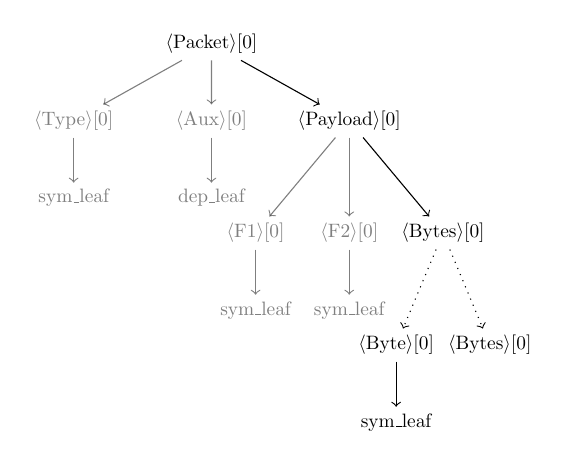
\begin{tikzpicture}[
    scale=0.7, transform shape,
    level distance=14mm,
    % root children (Type, Aux, Payload)
    level 1/.style={sibling distance=25mm},
    % children of Payload (F1, F2, Bytes)
    level 2/.style={sibling distance=17mm},
    % children of Bytes (Byte, Bytes)
    level 3/.style={sibling distance=17mm},
    baseline=(current bounding box.center),
  ]
    \node {$\langle$Packet$\rangle[0]$} [-to]
      child[opacity=.5] { node {$\langle$Type$\rangle[0]$}
        child { node {sym\_leaf} }}
      child[opacity=.5] { node {$\langle$Aux$\rangle[0]$}
        child { node {dep\_leaf} } }
      child { node {$\langle$Payload$\rangle[0]$} 
        child[opacity=.5] { node[yshift=-18pt] {$\langle$F1$\rangle[0]$} 
          child { node {sym\_leaf} } }
        child[opacity=.5] { node[yshift=-18pt] {$\langle$F2$\rangle[0]$} 
          child { node {sym\_leaf} }}
        child { node[yshift=-18pt] {$\langle$Bytes$\rangle[0]$} 
          % shift children of Bytes down to elongate arrows
          child[-to,dotted] { node[yshift=-18pt] {$\langle$Byte$\rangle[0]$}
            % this edge stays solid 
            child[-to,solid] { node {sym\_leaf} } }
          child[-to,dotted] { node[yshift=-18pt] {$\langle$Bytes$\rangle[0]$} } }
      };
  \end{tikzpicture}%
}
\resizebox{\textwidth}{!}{%
  \begin{tabular}{c c} 
    \blue{$\mathsf{packet0\_payload0\_bytes0\_opt0} >_{bv} 0x0$} & \dttreee 
  \end{tabular}
  % \dttreee
}
\end{frame}

% \begin{frame} \frametitle{Search Algorithm: Main concepts}
%     There are wrinkles...

%     \begin{enumerate}

%     \item Constraints must be \green{disambiguated} and \green{universalized}

%     \item Constraints may not be \green{applicable} 
%     \begin{itemize}
%       \item Extra constraint set \blue{$C$} to store inapplicable constraints
%       \item They may become applicable with future expansions! 
%       \item Remove \blue{$c$} from \blue{$C$} when its production rule instance has been backtracked
%     \end{itemize}
%     \end{enumerate}
% \end{frame}

\begin{frame}[fragile] \frametitle{Search Algorithm: Main concepts}
    There are wrinkles...
\vspace{-4pt}
    \begin{enumerate}
    % \item Constraints must be \green{disambiguated} and \green{universalized}
    \item[2.] This constraint is not \green{applicable}!
    \vspace{-4pt}
    \begin{itemize}
      \item Can it be applicable after a future decision? 
      \item Extra constraint set \blue{$C$} to store inapplicable constraints
      \item Remove from \blue{$C$} when backtracking
    \end{itemize}
    \end{enumerate}
\newcommand{\dttreee}{%
  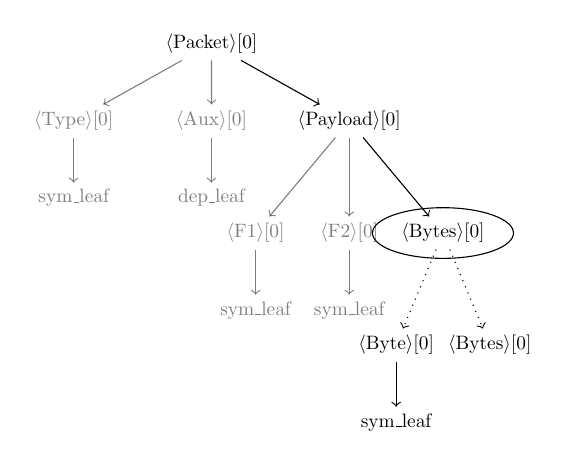
\begin{tikzpicture}[
    scale=0.7, transform shape,
    level distance=14mm,
    % root children (Type, Aux, Payload)
    level 1/.style={sibling distance=25mm},
    % children of Payload (F1, F2, Bytes)
    level 2/.style={sibling distance=17mm},
    % children of Bytes (Byte, Bytes)
    level 3/.style={sibling distance=17mm},
    baseline=(current bounding box.center),
  ]
    \node {$\langle$Packet$\rangle[0]$} [-to]
      child[opacity=.5] { node {$\langle$Type$\rangle[0]$}
        child { node {sym\_leaf} }}
      child[opacity=.5] { node {$\langle$Aux$\rangle[0]$}
        child { node {dep\_leaf} } }
      child { node {$\langle$Payload$\rangle[0]$} 
        child[opacity=.5] { node[yshift=-18pt] {$\langle$F1$\rangle[0]$} 
          child { node {sym\_leaf} } }
        child[opacity=.5] { node[yshift=-18pt] {$\langle$F2$\rangle[0]$} 
          child { node {sym\_leaf} }}
        child { node[yshift=-18pt,name=bytesnode] {$\langle$Bytes$\rangle[0]$} 
          child[-to,dotted] { node[yshift=-18pt] {$\langle$Byte$\rangle[0]$}
            child[-to,solid] { node {sym\_leaf} } }
          child[-to,dotted] { node[yshift=-18pt] {$\langle$Bytes$\rangle[0]$} } }
      }; 

  \node[draw, ellipse, fit=(bytesnode), inner sep=.5pt] {};
  \end{tikzpicture}%
}
\resizebox{\textwidth}{!}{%
  \begin{tabular}{c c} 
    \blue{$\mathsf{packet0\_payload0\_bytes0\_opt0} >_{bv} 0x0$} & \dttreee 
  \end{tabular}
  % \dttreee
}
\end{frame}


\begin{frame}
    \frametitle{Formal guarantees}
    In the paper, we formalize the \system{} search procedure as a calculus comprised of 11 inference rules \\[8pt] \pause

    We prove the calculus satisfies \green{solution soundness}, \green{refutation soundness}, 
    and \green{solution completeness}     
\end{frame}

\begin{frame}
    \frametitle{Evaluation}
    Case study 1, 2, 3: Compare directly with prior work, ISLa\pause
    \begin{itemize}
        \item XML, ScriptSize C, and CSV input generation \pause
        \item Matching tags, definition before use, and column count\pause
        \item Measure \green{efficiency} in inputs generated per minute and \green{diversity}
        in \green{k-path coverage} for \blue{$k=3$} (percentage of paths of length $3$ traversed through the grammar)\pause
        \item Outperform prior work by \blue{$\sim$$10-100\%$} in all metrics, save for efficiency of CSV inputs
    \end{itemize}
\end{frame}

\begin{frame}
    \frametitle{Evaluation}
    Case study 4\pause
    \begin{itemize}
        \item WiFi SAE packet input generation (SAECRED's SyGuS engine; \system{} predecessor) \pause
        \item Handle \green{bit vector SMT constraints} not expressible in ISLa \pause
        \item 36x improvement in efficiency \pause
        \item Able to produce outputs for more than twice the number of grammars 
        (\blue{$\sim$24,000 / $\sim$97000} up to \blue{$\sim$49,000 / $\sim$97,000})
    \end{itemize}
    % Comparison w/ ISLa: XML, ScriptSize C, and CSV
    %   Main metric are __efficiency__ in inputs/minute and __diversity__ in k-path coverage (define)
    %   Outperform prior work in the ballpark of 20-30 percentage points 
    %   in all metrics save for efficiency in CSV performance
    % Comparison w/ SAECRED
    %   36x faster 
    %   Can produce outputs for more than twice the inputs (~24,000 -> ~49,000 / ~97,000)
\end{frame}

\begin{frame}
    \frametitle{Discussion and future work}
    \begin{itemize}
        \item User-facing language 
        \begin{itemize} 
        \item \green{Synthesized} and \green{inherited attributes}
        \item User-defined \green{recursive functions} 
        \item Built-ins like \blue{{\scriptsize\texttt{length(.)}}}
        \end{itemize} \pause
        \item More powerful type system (e.g., \green{polymorphism})\pause
        \item AI \green{abstraction/refinement} algorithms\pause
        \item \green{Finite model finding} and \green{CLP} engines \pause
        \item \green{Divide and conquer/parallel} approaches \pause
        \item CDCL-style \green{backjumping}
    \end{itemize}
    % e.g., CLP semantics
\end{frame}

\begin{frame}
\center 
{\huge Thanks! Questions?}\\[12pt]

robert-lorch@uiowa.edu

\texttt{github.com/lorchrob/goblin}
\end{frame}

%%% End of presentation

\begin{frame}[fragile]
Every element of the second list is present in the first
    \frametitle{Structural constraints}
\begin{lstlisting}[style=goblin]
@\color{darkred}<S>@ ::= @\color{darkred}<L1> <L2>@
      { @\color{darkred}<L2>@.@\color{teal}<\_defs\_down>@ = @\color{darkred}<L1>@.@\color{teal}<\_defs\_up>@; };
@\color{darkred}<L1>@ ::= @\color{teal}<\_defs\_up> <str>@ @\color{darkred}<L1>@
       { @\color{teal}<\_defs\_up>@ = set.union(set.singleton(@\color{teal}<str>@), 
                                @\color{darkred}<L1>@.@\color{teal}<\_defs\_up>@); }
       | @\color{teal}<\_defs\_up>@ @\color{darkred}<str>@
       { @\color{teal}<\_defs\_up>@ = set.singleton(@\color{teal}<str>@); };
@\color{darkred}<L2>@ ::= @\color{teal}<\_defs\_down> <str>@ @\color{darkred}<L2>@ 
       { set.member(@\color{teal}<str>@, @\color{teal}<\_defs\_down>@); 
         @\color{darkred}<L2>@.@\color{teal}<\_defs\_down>@ = @\color{teal}<\_defs\_down>@; }
       | @\color{teal}<\_defs\_down> <str>@
       { set.member(@\color{teal}<str>@, @\color{teal}<\_defs\_down>@); };
@\color{teal}<str>@ :: String;
@\color{teal}<\_defs\_down>@ :: Set(String); 
@\color{teal}<\_defs\_up>@ :: Set(String);
\end{lstlisting}
\end{frame}

\begin{frame} 
    \frametitle{Prior Work} 
    \begin{itemize}
        \item ISLa, most similar in spirit 
        \begin{itemize}
            \item Only natively supports string constraints
            \item Global constraints not amenable to \green{grammar mutations}
        \end{itemize}
        \item Fandango
    \begin{itemize}
        \item Uses  \green{genetic algorithms} with built-in fitness functions
        \item Constraints may be \green{non-monotonic} (no monotonically decreasing notion of distance for constraint satisfaction)
        \item Times out for simple examples (equality, set membership)
        \item Times out with SAECRED grammars
    \end{itemize}
    \end{itemize}
\end{frame}

\begin{frame} 
    \frametitle{Related Work} 
    \begin{itemize}
        \item Parser generator libraries (e.g. ANTLR, yacc) handle context sensitivity 
        but are for \green{parsing} rather than generation
        \item Attribute grammars handle context sensitivity but work focuses on \green{parsing} and theoretical results
        \item Property-based testing does not support \green{general context-sensitive constraints} over inputs
        \item SyGuS does not natively support \green{constraints over non-top-level nonterminals} 
    \end{itemize}
    
    % Why build a new input generation tool? How do we position ourselves compared to prior work?
    % There are two prior works that target the same question
    % First, ISLa:
    % (i)  integration with fuzzing workflows -- philosophically, local constraints (example)
    % (ii) re-conceptualizing the problem to craft a semantics that natively supports diverse datatypes
    %         - ADT term generator, not a string generator
    %         - give an example of ADT vs string distinction
    % (iii) minimal core language without sacrificing expressiveness
    %         - clarify formal foundations
    %         - simplify implementation
    %         - avoid special cases
    %         - pave the way for future work (surface-level DSL)
    % Fandango:
    % * No constraint solving, genetic algorithms
    % * How to come up with a fitness function?
    % * Constraints can be nonmonotonic
    % * Killed by simple examples (give examples)
\end{frame}

\begin{frame}[fragile]
    \frametitle{Local constraints for grammar mutation}
\begin{itemize}
    \item \green{Crossover mutation} swapping {\scriptsize\texttt{GROUP\_ID}} and {\scriptsize\texttt{RG\_LIST}}
    \item \green{Local constraints} are easier to maintain
\end{itemize}

\begin{lstlisting}[style=plain]
COMMIT ::= SEQ GROUP_ID SCALAR
  { GROUP_ID is equal to 13  and  SEQ is greater than 4 }
RG_CONT ::= RG_LENGTH RG_TY RG_LIST
  { RG_LENGTH is the length of RG_LIST }
...
-->
COMMIT ::= SEQ RG_LIST SCALAR
  { SEQ is greater than 4 }
RG_CONT ::= RG_LENGTH RG_TY GROUP_ID
  { GROUP_ID is equal to 13 }
...
\end{lstlisting}
\end{frame}

\begin{frame}
    \frametitle{Semantics: Interpretation function}
Interpretation function \blue{$\mathcal{I}_{\mathit{tr}}(t)$} outputs denotation 
of term \blue{$t$} in AST \blue{\emph{tr}} \\[4pt]

\blue{$\mathcal{I}_{tr}$} also maps function and predicate symbols 
to their fixed interpretations\\[4pt]

\blue{{\small\noindent$
\begin{array}{ll} 
&\mathcal{I}_{tr}(f(t_1, \dots, t_n)) = \top \text{ if some } \mathcal{I}_{tr}(t_i) = \top  \\
&\mathcal{I}_{tr}(f(t_1, \dots, t_n)) = \mathcal{I}_{tr}(f)(\mathcal{I}_{tr}(t_1), \dots, \mathcal{I}_{tr}(t_n)) \\
&\mathcal{I}_{tr}(\nt{nt}[i].\nt{nt\_expr}) = \mathcal{I}_{tr'}(\nt{nt\_expr}) \text{ for } \mathit{tr}' \text{ rooted at the only } \\
    &\;\;\;\;\;\;v \in \mathsf{get\_children(\mathit{tr}, root(}\mathit{tr})) \text{ such that } \ell(v) = \nt{nt}[i] \\
    &\dots
\end{array}
$}}
\end{frame}

\begin{frame} 
    \frametitle{Semantics: Satisfaction relation}
Satisfaction relation \blue{$\models_{\mathcal{G}}$} captures whether or not a given constraint in \blue{$G$}
is satisfied by a given AST\\[4pt]

\blue{
  \(
\begin{array}{l}
    \mathit{tr} \models_{\mathcal{G}} \varphi \text{ if } \mathcal{I}_{\mathit{tr}}(t_i) = \top \text{ for some subterm } t_i \text{ of } \varphi \text{; otherwise,} \\
    \mathit{tr} \models_{\mathcal{G}} p(t_1, \dots, t_n) \text{ if } (\mathcal{I}_{tr}(t_1), \dots, \mathcal{I}_{tr}(t_n)) \in \mathcal{I}_{tr}(p) \\
    \mathit{tr} \models_{\mathcal{G}} \neg \varphi \text{ if } \mathit{tr} \not\models_{\mathcal{G}} \varphi \\
    \mathit{tr} \models_{\mathcal{G}} \varphi_1 \land \varphi_2 \text{ if } \mathit{tr} \models_{\mathcal{G}} \varphi_1 \text{ and } \mathit{tr} \models_{\mathcal{G}} \varphi_2 \\
    \mathit{tr} \models_{\mathcal{G}} \varphi_1 \lor \varphi_2 \text{ if } \mathit{tr} \models_{\mathcal{G}} \varphi_1 \text{ or } \mathit{tr} \models_{\mathcal{G}} \varphi_2 \\
    \mathit{tr} \models_{\mathcal{G}} \varphi_1 \Rightarrow \varphi_2 \text{ if } \mathit{tr} \not\models_{\mathcal{G}} \varphi_1 \text{ or } \mathit{tr} \models_{\mathcal{G}} \varphi_2 \\
\end{array}
\)}
\end{frame}

\begin{frame} 
    \frametitle{Semantics: Denotation of $G$}
Semantics of a \system{} input \blue{$G$} is the set of syntactically valid ASTs 
which satisfy all the constraints

\blue{
{\small
\begin{align*}
\llbracket G \rrbracket = 
    \{ t \mid \; &t \in \mathcal{L}_{\mathsf{AST}}(G) \land \forall (\textsf{nt}, \_, \textsf{constraints}) \in R.\; \\[-1ex]
              &\forall s \in \textsf{get\_subtrees}(t, \textsf{nt}). \; 
              \forall \varphi \in \textsf{constraints}. \; 
              \mathit{s} \models_{\mathcal{G}} \textsf{resolve}(\varphi)    
    \}  
\end{align*}
}}
\end{frame}



\begin{frame} 
    \frametitle{Calculus}
Can conceptualize as \green{guarded rewrite rules} on global state\\[4pt]

Example rule expands a symbolic terminal

\centering
\blue{\begin{mathpar} 
  \inferrule*[left=NormalizeTA]
% v is an open leaf in the derivation tree DT
% label of v is associated with type annotation ta carrying semantic constraint set D
  { v \in \mathsf{open\_leaves}(DT) \quad 
    \mathsf{depth}(\mathit{DT}) \leq L \quad 
    \ell(v), \tau \in \Gamma }
% add D to set of constraints C
% still expand DT' so we know we already colelcted this constraint
  { \mathit{DT}' \gets \mathsf{expand}_G(\mathit{DT}, v, []) }
\end{mathpar}}
\end{frame}

\begin{frame}
    \frametitle{Search algorithm pseudocode}
    
  {\tiny
  \begin{algorithmic}[1]
    \raggedright
    \STATE $\texttt{initializeGlobalState}()$
    % \STATE $\func{push}(\mathsf{decisionStack}, \mathtt{stNode})$
      \WHILE{$\lnot \func{allLeavesClosed}(\mathit{dt})$}
        \IF{\text{there is more than one unvisited expansion}}
          \STATE $\textsc{Decide}$
        \ELSE
          \STATE $\textsc{Propagate}$
        \ENDIF

        \WHILE{$\lnot \mathsf{is\_normalized}(\mathit{dt})$}
          \STATE $\textsc{NormalizePr}$ \text{ (if applicable)}
          \STATE $\textsc{NormalizeTa}$ \text{ (if applicable)}
        \ENDWHILE

        \IF{\textnormal{current search depth } d > \textnormal{depth limit } L}
          \IF{$\mathsf{assertionLevel} = 1$}
            \STATE $\textsc{RestartDepth}$
          \ELSE
            \STATE $\textsc{BacktrackDepth}$
          \ENDIF
        \ELSE
          \FORALL{$c \in \textnormal{constraint set } C$}
            \STATE \textsc{Assert} \text{ if } c \text{ is applicable}
          \ENDFOR
          \IF{$\func{smt\_check\_sat}() = \mathsf{UNSAT}$}
            \IF{$\mathsf{assertionLevel} = 1 \land \lnot \mathit{bd?}$}
              \STATE $\textsc{Fail}$
            \ELSIF{$\mathsf{assertionLevel} = 1$}
              \STATE $\textsc{RestartUnsat}$
            \ELSE
              \STATE $\textsc{BacktrackUnsat}$
            \ENDIF
          \ENDIF
        \ENDIF
      \ENDWHILE
  \end{algorithmic}}
\end{frame}


\end{document}

%!! Callouts
%.   Generality of CFGs with expressivity of tailor-made tools
%.   Term generation view gives flexibility of ADTs, including at the type level
%.   Local constraints align with CFG-level grammar mutations